\documentclass[10pt]{myland}

%%%%%%%%%%%%%%%%%%%%%%%%%%%%FILE TITLE%%%%%%%%%%%%%%%%%%%%%%%%%%%%%%%%%%%%
\begin{document}
\begin{center}
	{\Large \myhwname{CSE 444: Lab 3 Writeup}} \\
	\vspace{.05in}
    \myname{Linxing Preston Jiang}\quad\quarter{Winter 2018}\\
	\vspace{.05in}
    \today \\
\end{center}
\vspace{.15in} \hrule \vspace{0.5em}%


\begin{enumerate}[label=\textbf{\arabic*.}, listparindent=0.0em, itemsep=2em]
	\item
	Lab 3 focuses on adding Transactions functionality to simpleDB. Specifically, we implemented NO STEAL (never evict
    dirty pages from the buffer pool if they are locked by an uncommited transaction), and FORCE (on transaction commit,
    force write pages to disk) for buffer pool management. In order to achieve this, we implemented our own
    \texttt{Lock} and \texttt{LockManager} which together handle acquiring/releasing both \texttt{SHARED} (read-only)
    and \texttt{EXCLUSIVE} (read-write) locks by different transactions on page granularity. Another important part of
    transcations is deadlock detection and resolution. For lab3, I implemented time-out limits for \texttt{acquire} so
    that a certain period time of blocking on \texttt{acquire} will be considered as deadlock and thus abort the
    transaction. \par

    Main parts of lab3 include:
	\begin{itemize}
        \item \texttt{Lock}: We need this class to represent the two types of locks simpleDB uses: \texttt{SHARED} and
            \texttt{EXCLUSIVE}. A shared lock is acquired by read-only transactions, and thus can be shared between
            many read-only transactions; an exclusive lock is acquired by read-write transactions, and thus can only be
            acquired by at most one read-write transaction at a time.

        \item \texttt{LockManager}: We need this class as the manager for all locking-related actions in simpleDB. It
            is created within \texttt{BufferPool} and will be called to acquire locks when \texttt{getPage} is called
            and release locks when \texttt{transactionComplete} is called. Note that because of the design of simpleDB,
            \texttt{acquire} in \texttt{LockManager} should only need calling in \texttt{getPage} when simpleDB wants to
            interact with a page. For more about blocking and deadlock detection/resolution, see ``design'' part of this
            writeup.

        \item \texttt{BufferPool.transactionComplete}: We need this method to release all locks acquired by a
            transaction when it commits. Note that because we choose to implement \texttt{NO STEAL}, releasing locks
            should only happen at this method except aborting transactions.
	\end{itemize}

    \item I suggest adding a new unit test for the correctness of \texttt{BufferPool.flushPages}. More specifically,
        when flusing all the pages for committing a transaction, \texttt{BufferPool} should only flush pages which are
        dirtied by \textbf{\emph{this}} transaction, not just all dirty pages which are possibly marked dirty by other
        transactions that are not committing. An extra test on this behavior would be helpful for debugging.

    \item Design decisions:
        \begin{enumerate}
            \item Lock
                \begin{itemize}
                    \item Lock has two types: \texttt{SHARED} or \texttt{EXCLUSIVE}.
                    \item Lock keeps a hash set of \texttt{TransactionIds}, mainly for shared locks to keep track of
                        it is shared by which transactions.
                    \item Lock is used to ensure \textbf{page} granularity.
                \end{itemize}
            \item LockManager
                \begin{itemize}
                    \item LockManager is implemented as Singleton, for there should be only one object of
                        \texttt{LockManager} to manage all transactions, just like \texttt{BufferPool}.
                    \item Lock keeps a hash map from \texttt{TransactionId} to a hash set of \texttt{PageIds} to keep
                        track of which pages a certain transaction has locks on. It also keeps a hash map from \texttt{PageId}
                        to \texttt{Lock}.
                    \item There are a few conditions when \texttt{acquire} will not be a blocking call. They are:
                        \begin{itemize}
                            \item When the lock on that page is not locked.
                            \item When the lock is locked by this transaction itself (will upgrade a share lock to
                                exclusive if this transaction is the only one which holds the lock)
                            \item When the lock is locked, but it is a shared lock, and the transaction wants a shared lock.
                        \end{itemize}
                    \item When \texttt{acquire} is a blocking call, the transaction will sleep for 500 milliseconds, and
                        then it will try to acquire for the lock again. If the second try still fails, it will be
                        considered as a deadlock condition, and so \texttt{acquire} throws a \texttt{TransactionAbortedException}.
                \end{itemize}
            \item BufferPool
                \begin{itemize}
                    \item
                \end{itemize}
        \end{enumerate}

    \newpage
    \par Examples:
    \par Workflow (\texttt{join()}, showing \texttt{next()} call): \\
    \begin{center}
        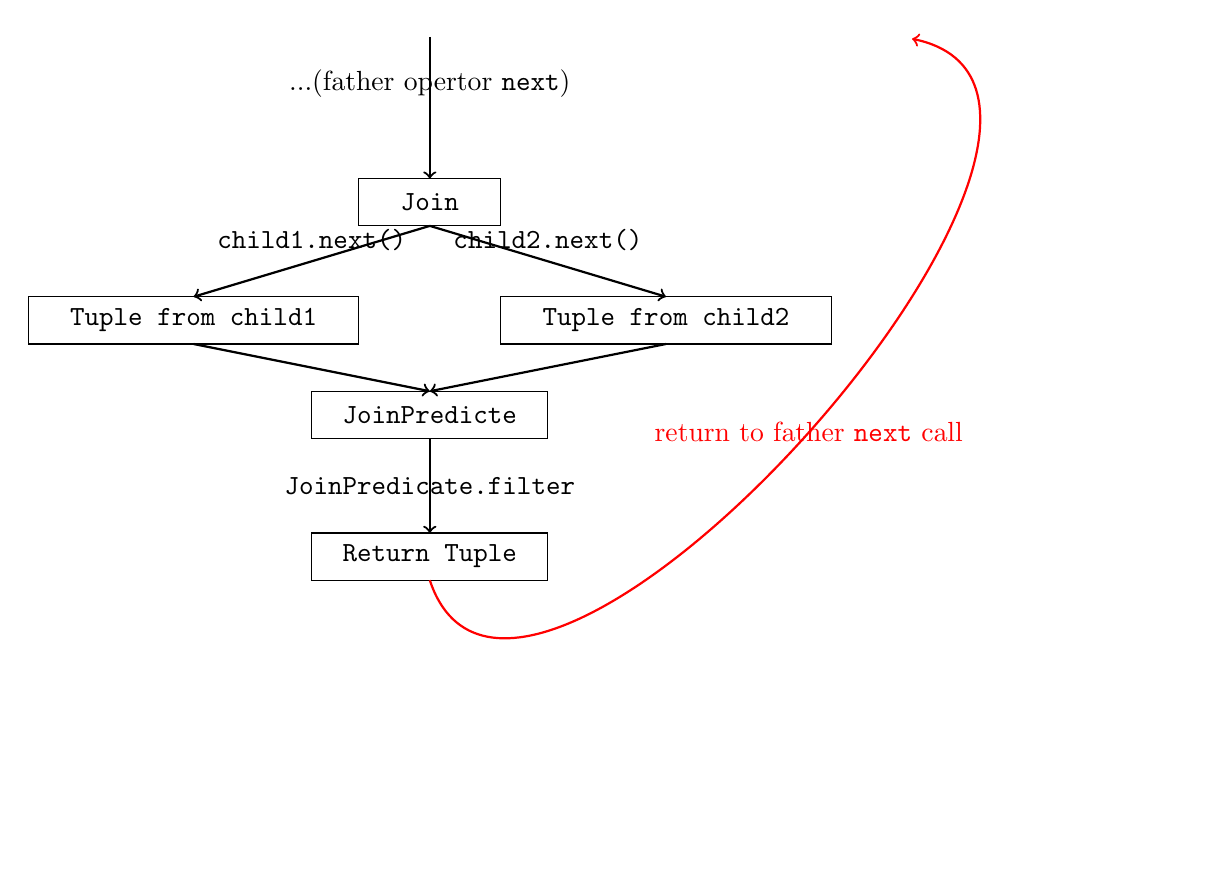
\begin{tikzpicture}[
            scale=.6,
        ]
            \path[->, thick] (0, 3) edge node[midway, above] {...(father opertor \texttt{next})} (0, 0);
            \draw[draw=black] (-1.5, 0) rectangle (1.5, -1) node[midway]  {\texttt{Join}};
            \path[->, thick] (0, -1) edge node[midway, above] {\texttt{child1.next()}} (-5, -2.5);
            \path[->, thick] (0, -1) edge node[midway, above] {\texttt{child2.next()}} (5, -2.5);
            \draw[draw=black] (-8.5, -2.5) rectangle (-1.5, -3.5) node[midway]  {\texttt{Tuple from \texttt{child1}}};
            \draw[draw=black] (1.5, -2.5) rectangle (8.5, -3.5) node[midway]  {\texttt{Tuple from \texttt{child2}}};
            \path[->, thick] (-5, -3.5) edge node[midway, above] {} (0, -4.5);
            \path[->, thick] (5, -3.5) edge node[midway, above] {} (0, -4.5);
            \draw[draw=black] (-2.5, -4.5) rectangle (2.5, -5.5) node[midway]  {\texttt{JoinPredicte}};
            \path[->, thick] (0, -5.5) edge node[midway] {\texttt{JoinPredicate.filter}} (0, -7.5);
            \draw[draw=black] (-2.5, -7.5) rectangle (2.5, -8.5) node[midway]  {\texttt{Return Tuple}};
            \node (father) at (10, 3) {};
            \path[->, thick, color=red] (0, -8.5) edge [bend right=120] node[midway] {return to father \texttt{next} call} (father);
        \end{tikzpicture}
    \end{center}
    Workflow (\texttt{insertTuple()}): \\
    \begin{center}
        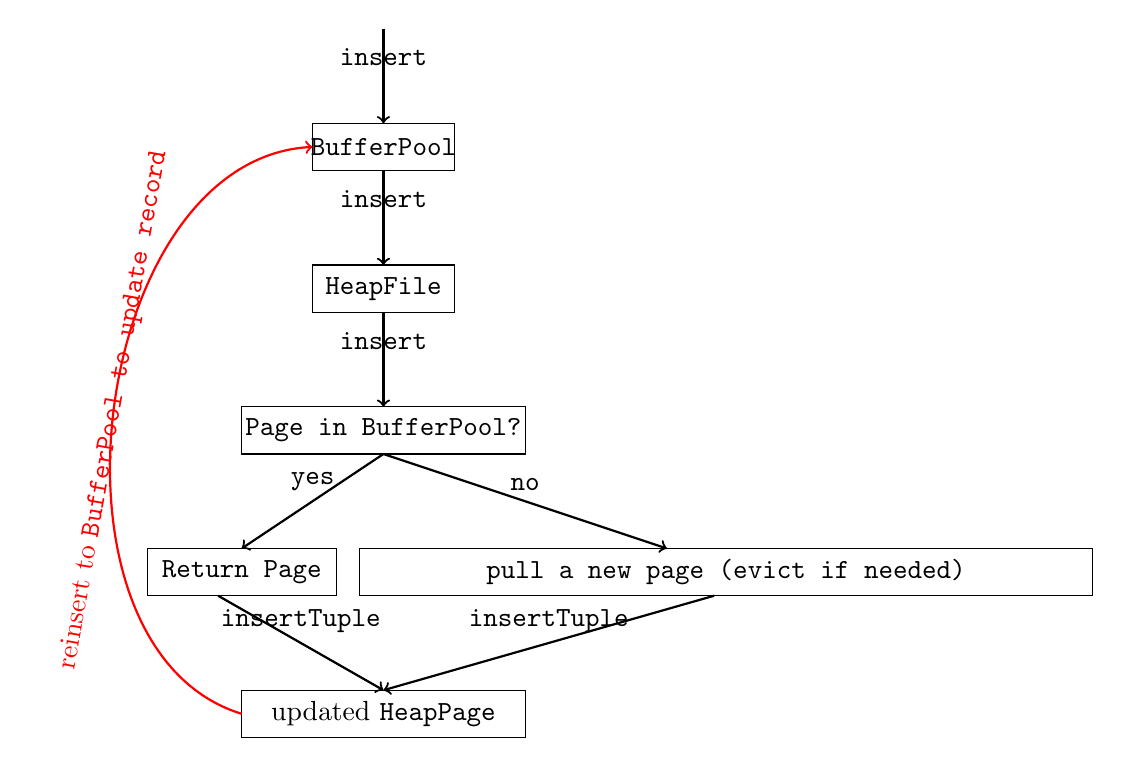
\begin{tikzpicture}[
            scale=.6,
        ]
            \path[->, thick] (0, 2) edge node[midway, above] {\texttt{insert}} (0, 0);
            \draw[draw=black] (-1.5, 0) rectangle (1.5, -1) node[midway]  {\texttt{BufferPool}};
            \path[->, thick] (0, -1) edge node[midway, above] {\texttt{insert}} (0, -3);
            \draw[draw=black] (-1.5, -3) rectangle (1.5, -4) node[midway]  {\texttt{HeapFile}};
            \path[->, thick] (0, -4) edge node[midway, above] {\texttt{insert}} (0, -6);
            \draw[draw=black] (-3, -6) rectangle (3, -7) node[midway]  {\texttt{Page in BufferPool?}};
            \path[->, thick] (0, -7) edge node[midway, above] {\texttt{yes}} (-3, -9);
            \path[->, thick] (0, -7) edge node[midway, above] {\texttt{no}} (6, -9);
            \draw[draw=black] (-5, -9) rectangle (-1, -10) node[midway]  {\texttt{Return Page}};
            \draw[draw=black] (-0.5, -9) rectangle (15, -10) node[midway]  {\texttt{pull a new page (evict if needed)}};
            \path[->, thick] (-3.5, -10) edge node[midway, above] {\texttt{insertTuple}} (0, -12);
            \path[->, thick] (7, -10) edge node[midway, above] {\texttt{insertTuple}} (0, -12);
            \draw[draw=black] (-3, -12) rectangle (3, -13) node[midway]  {updated \texttt{HeapPage}};
            \path[->, thick, color=red] (-3, -12.5) edge [bend left=80] node[midway, rotate=80] {reinsert to \texttt{BufferPool
                to update record}} (-1.5, -0.5);
        \end{tikzpicture}
    \end{center}
    \newpage

    \item Design decisions: I chose to use nested loop join. Nested-loop-join is the slowest but it works for all kinds
        of comparisons (Hash join only works well for equality comparison, sort-merge join only works well for inequaliy
        comparison). For eviction policy, I chose to evict the first page every time the \texttt{BufferPool} is full.
        This does not work well in terms of keeping most commonly used page in memory, which result in extra disk IOs,
        but the implementation is easy and does not require extra data structures in order to keep track of page usage.

    \item Extra Unit tests: A unit test for the correctness of HeapFile insertTuple behavior would be great. The spec
        requires the update of \texttt{BufferPool} pages to happen in the insert/delete methods of \texttt{BufferPool}
        instead of in \texttt{HeapFile}. I did it the wrong way and caused the \texttt{handleManyDirty} test to fail, and
        it took me a while to realize that test uses a overriden \texttt{insert} method and \texttt{BufferPool} should
        be in charge of updating the record.

    \item Changes to API: I did not make changes to the APIs given.

    \item Missing elements: I believe I finished the entire Lab 2
\end{enumerate}
\end{document}
